\documentclass[12pt]{article}
%%%%%%%%%%%%%%%%%%%%%%%%%%%%%%%%%%%%%%%%%%%%%%%%%%%%%%%%%%%%%
%% Document setup for Syllabus and HW

\textwidth=7in
\textheight=9.5in
\topmargin=-1in
\headheight=0in
\headsep=.5in
\hoffset  -.85in

\usepackage{amsmath} % for \text{}
\usepackage{amsfonts} % For \text{}
\usepackage{amssymb} % For \text{}
\usepackage{nth}
\usepackage{enumerate}
%\usepackage{nth}

%% Stolen from Nathan Baker
\newcommand{\erf}{{\mathrm{erf}}}
\newcommand{\erfc}{{\mathrm{erfc}}}
\newcommand{\erfi}{{\mathrm{erfi}}}
\newcommand{\argh}{{\mathrm{arg}}}
\newcommand{\atan}{{\mathrm{atan}}}
\newcommand{\acos}{{\mathrm{acos}}}
\newcommand{\asin}{{\mathrm{asin}}}
\newcommand{\mat}[1]{\,\underline{\underline{#1}}\,}
\newcommand{\abs}[1]{\left| #1 \right|}
\newcommand{\norm}[1]{\left\| #1 \right\|}
\newcommand{\order}[1]{{\mathcal{O}} \left( #1 \right)}
\newcommand{\op}[1]{{\mathcal{#1}}}
\newcommand{\myfile}[1]{\texttt{#1}}
\newcommand{\myvar}[1]{\textsf{#1}}
\newcommand{\mean}[1]{{\left\langle {#1} \right\rangle}}

% The master boolean -- set this to "masterfalse" or "mastertrue"
%\newif\ifmaster \masterfalse
\newif\ifmaster \masterfalse
\newif\ifmaster \mastertrue

%http://tex.stackexchange.com/questions/145812/using-fbox-in-a-newenvironment
\newcommand\notes[1]{%
  \fbox{\begin{minipage}{0.9\textwidth}#1\end{minipage}}}

%%\newcommand{\hidesolution}[1]{ \ifmaster { {#1} } \else { {Go to class.} } \fi }
%%\newcommand{\hideanswer}[1]{ \ifmaster { #1 } \else {} \fi }
%%\newcommand{\solution}[1]{ \begin{proof}[Solution] \hidesolution{#1} \end{proof} }
%%\newcommand{\answer}[1]{ \hideanswer{\newpage\ \newpage \notes{\begin{proof}[Answer] #1 \end{proof}}} }

%% MGL
\newcommand{\CC}{\mathbb{C}}
\newcommand{\N}{\mathbb{N}}
%\newcommand{\vect}[1]{\,\vec{\mathbf{#1}}\,}
\newcommand{\vect}[1]{\,\mathbf{#1}\,}
\usepackage{tabularx}
\newcommand{\vtau}{\vect{\tau}}
\newcommand{\va}{\vect{a}}
\newcommand{\vb}{\vect{b}}
\newcommand{\vc}{\vect{c}}
\newcommand{\vd}{\vect{d}}
\newcommand{\ve}{\vect{e}}
\newcommand{\vf}{\vect{f}}
\newcommand{\vg}{\vect{g}}
\newcommand{\vh}{\vect{h}}
\newcommand{\vi}{\vect{i}}
\newcommand{\vj}{\vect{j}}
\newcommand{\vk}{\vect{k}}
\newcommand{\vl}{\vect{l}}
\newcommand{\vm}{\vect{m}}
\newcommand{\vn}{\vect{n}}
\newcommand{\vo}{\vect{o}}
\newcommand{\vp}{\vect{p}}
\newcommand{\vq}{\vect{q}}
\newcommand{\vr}{\vect{r}}
\newcommand{\vs}{\vect{s}}
\newcommand{\vt}{\vect{t}}
\newcommand{\vu}{\vect{u}}
\newcommand{\vv}{\vect{v}}
\newcommand{\vw}{\vect{w}}
\newcommand{\vx}{\vect{x}}
\newcommand{\vy}{\vect{y}}
\newcommand{\vz}{\vect{z}}

\newcommand{\vA}{\vect{A}}
\newcommand{\vB}{\vect{B}}
\newcommand{\vC}{\vect{C}}
\newcommand{\vD}{\vect{D}}
\newcommand{\vE}{\vect{E}}
\newcommand{\vF}{\vect{F}}
\newcommand{\vG}{\vect{G}}
\newcommand{\vH}{\vect{H}}
\newcommand{\vI}{\vect{I}}
\newcommand{\vJ}{\vect{J}}
\newcommand{\vK}{\vect{K}}
\newcommand{\vL}{\vect{L}}
\newcommand{\vM}{\vect{M}}
\newcommand{\vN}{\vect{N}}
\newcommand{\vO}{\vect{O}}
\newcommand{\vP}{\vect{P}}
\newcommand{\vQ}{\vect{Q}}
\newcommand{\vR}{\vect{R}}
\newcommand{\vS}{\vect{S}}
\newcommand{\vT}{\vect{T}}
\newcommand{\vU}{\vect{U}}
\newcommand{\vV}{\vect{V}}
\newcommand{\vW}{\vect{W}}
\newcommand{\vX}{\vect{X}}
\newcommand{\vY}{\vect{Y}}
\newcommand{\vZ}{\vect{Z}}
\newcommand{\diffd}{\mathrm{d}}
\newcommand{\deriv}[2]{\frac{\diffd #1}{\diffd #2}} % derivative
%\newcommand{\pd}[2]{\frac{\partial#1}{\partial#2}}
%\newcommand{\dd}[2]{\frac{d#1}{d#2}}
\newcommand{\dinline}[2]{\diffd #1/\diffd #2} % for derivatives
\newcommand{\pdinline}[2]{\partial#1/\partial#2}

%\newcommand{\bra}[1]{\left\langle #1 \right|}
%\newcommand{\ket}[1]{\left| #1 \right\rangle}

\newcommand{\xd}{\dot{x}}

\newcommand{\boldcent}[1] {\begin{center}\textbf{ #1 }\end{center}}
% ***********************************************************
% ******************* PHYSICS HEADER ************************
% ***********************************************************
% From http://www.dfcd.net/articles/latex/latex.html
% Version 2
%\documentclass[11pt]{article} 
\usepackage{amsmath} % AMS Math Package
\usepackage{amsthm} % Theorem Formatting
\usepackage{amssymb}	% Math symbols such as \mathbb
\usepackage{graphicx} % Allows for eps images
\usepackage{multicol} % Allows for multiple columns
%\usepackage[dvips,letterpaper,margin=0.75in,bottom=0.5in]{geometry}
% % Sets margins and page size
%\pagestyle{empty} % Removes page numbers
%\makeatletter % Need for anything that contains an @ command 
%\renewcommand{\maketitle} % Redefine maketitle to conserve space
%{ \begingroup \vskip 10pt \begin{center} \large {\bf \@title}
%	\vskip 10pt \large \@author \hskip 20pt \@date \end{center}
%  \vskip 10pt \endgroup \setcounter{footnote}{0} }
%\makeatother % End of region containing @ commands
\renewcommand{\labelenumi}{(\alph{enumi})} % Use letters for enumerate
% \DeclareMathOperator{\Sample}{Sample}
\let\vaccent=\v % rename builtin command \v{} to \vaccent{}
\renewcommand{\v}[1]{\ensuremath{\mathbf{#1}}} % for vectors
\newcommand{\gv}[1]{\ensuremath{\mbox{\boldmath$ #1 $}}} 
% for vectors of Greek letters
\newcommand{\uv}[1]{\ensuremath{\mathbf{\hat{#1}}}} % for unit vector
%\newcommand{\abs}[1]{\left| #1 \right|} % for absolute value
\newcommand{\avg}[1]{\left< #1 \right>} % for average
\let\underdot=\d % rename builtin command \d{} to \underdot{}
\newcommand{\fd}[2]{\frac{d #1}{d #2}} % for derivatives
\newcommand{\dd}[2]{\frac{d^2 #1}{d #2^2}} % for double derivatives
\newcommand{\pd}[2]{\frac{\partial #1}{\partial #2}} 
% for partial derivatives
\newcommand{\pdd}[2]{\frac{\partial^2 #1}{\partial #2^2}} 
% for double partial derivatives
\newcommand{\pdc}[3]{\left( \frac{\partial #1}{\partial #2}
 \right)_{#3}} % for thermodynamic partial derivatives
\newcommand{\ket}[1]{\left| #1 \right>} % for Dirac bras
\newcommand{\bra}[1]{\left< #1 \right|} % for Dirac kets
\newcommand{\braket}[2]{\left< #1 \vphantom{#2} \right|
 \left. #2 \vphantom{#1} \right>} % for Dirac brackets
\newcommand{\matrixel}[3]{\left< #1 \vphantom{#2#3} \right|
 #2 \left| #3 \vphantom{#1#2} \right>} % for Dirac matrix elements
\newcommand{\grad}[1]{\gv{\nabla} #1} % for gradient
\let\divsymb=\div % rename builtin command \div to \divsymb
\renewcommand{\div}[1]{\gv{\nabla} \cdot #1} % for divergence
\newcommand{\curl}[1]{\gv{\nabla} \times #1} % for curl
\let\baraccent=\= % rename builtin command \= to \baraccent
\renewcommand{\=}[1]{\stackrel{#1}{=}} % for putting numbers above =
\newtheorem{prop}{Proposition}
\newtheorem{thm}{Theorem}[section]
\newtheorem{lem}[thm]{Lemma}
\theoremstyle{definition}
\newtheorem{dfn}{Definition}
\theoremstyle{remark}
\newtheorem*{rmk}{Remark}

% ***********************************************************
% ********************** END HEADER *************************
% ***********************************************************

\usepackage{nth}
%%%%%%%%%%%%%%%%%%%%%%%%%%%%%%%%%%%%%%%%%%%%%%%%%%%%%%%%%%%%%
\pagestyle{empty}
\begin{document}
\begin{center}

\vskip.15in
\noindent\textbf{Assignment 7, Due Wednesday April \nth{13} by 11:00 AM}
\vskip.15in
\end{center}

\section{Finishing Green's Theorem}
\subsection{Finishing our in-class problem} We evaluated a line
integral around several paths in class. Use the parabola as the bottom
of a region, and the edges of the rectangle as the left side and top
fo the region, and explicitly verify Green's Theorem for the field
discussed in class.

\section{The wave equation}
\subsection{Additional problem} Argue that the wave equation is a
reasonable physical model for waves. You may make this argument for
1D, 2D, or 3D waves. Does it seem reasonable for both longitudinal and
transverse waves? You may use the book, the internet, or whatever
resources you'd like, but make sure to cite your sources.
\subsection{Boas \S13.1} Boas 13.1.2
\section{Diffusion/Heat Flow; Schrodinger}
\subsection{Boas \S13.2} 13.2.3, 13.2.7
\subsection{Boas \S13.3} 13.3.1; you must also write down the rest of the answer to Example 1. It's perfectly fine to use the book as a reference *before* you write you answer, but I want you to write it out in your final form without looking at the book.
\section{Steady State Temp in a Rectangular Plate}
\subsection{Additional problem} Most of the problems we've been solving involve an infinite number of terms in the solution. With appropriate boundary conditions, this is not required. Solve the semi-infinite rectangular plate problem with one side of the plate held at

\begin{equation}
  T = \sin\left(\frac{-2\pi x}{L}\right) + \cos\left(\frac{3\pi x}{L}\right)
\end{equation}

How many terms do you find in your solution, a finite number, or an infinite number? If it's finite, why should that be true conceptually? If it's infinite, why should that be true conceptually?

%also, I think that, as per the next problem, that one actually does have an infinite number of terms. But maybe not. Why not just sin(2x/L) if it's just the sin term? the infinite number must come from the discontinuity.

\section{FRAP (Adapted from ``Physical Biology of the Cell'', Ch. 13)}
In biology, one often wants to know how quickly various molecules are
moving. The standard way of performing these experiments under a wide
variety of experimental settings is with Fluorescence Recovery After
Photobleaching (FRAP). In the figure below\footnote{C. W. Mulineaux et
al., J. Baceriol. 188:3442,2006}, an elongated
\textit{E. coli} cell with TorA-GFP (a protein fused with green
fluorescent protein) is shown on the far left. A TorA-GPF loses its
fluorescent properties when you shine a strong laser on it
(``photobleaching''). In the second frame, you see an image of the
cell that has been photobleached at the site indicated by the
arrow. 

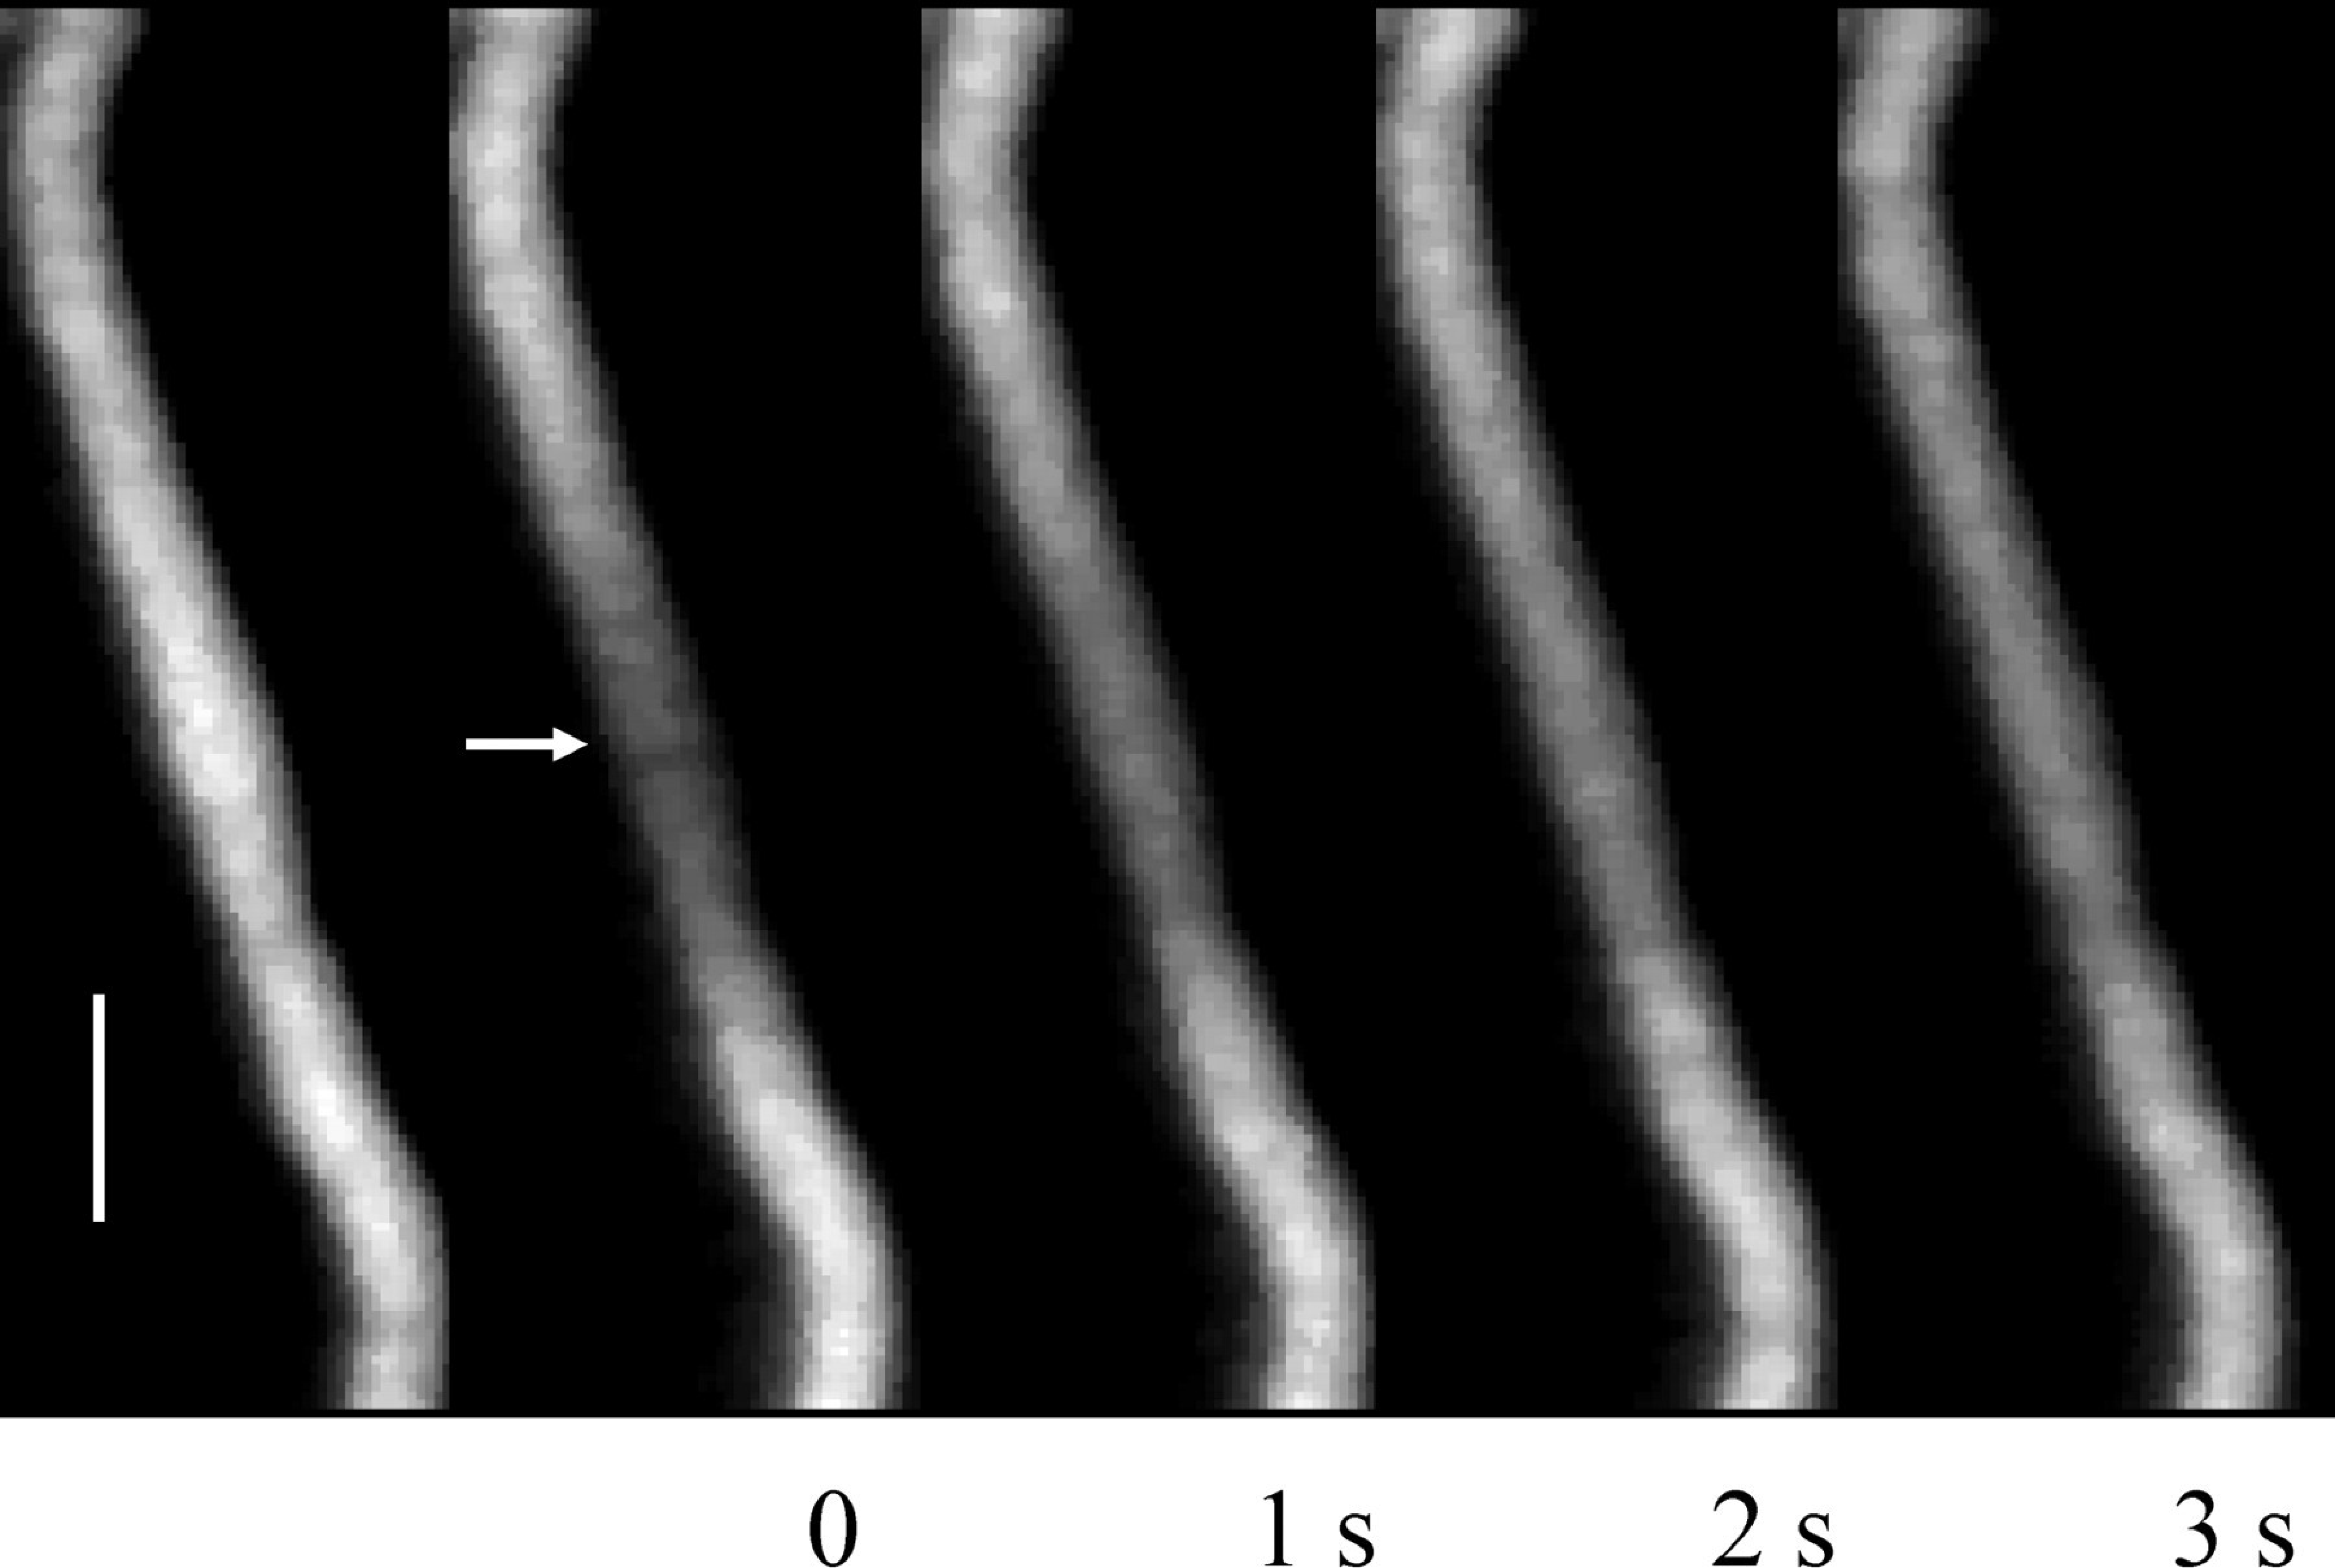
\includegraphics[height=50mm]{F5_large.pdf}

As fluorescent proteins from \textit{outside} that area diffuse
in (frames 1s to 3s), the bleached area becomes more fluorescent. By
measuring the rate at which the fluorescence returns, you can find out
how quickly the proteins are diffusing within the cell. The image
below shows the difference in fluorescence immediately after bleaching
(dark jagged line) and 4 seconds after (light jagged line), along with
fits to the data (smooth lines).

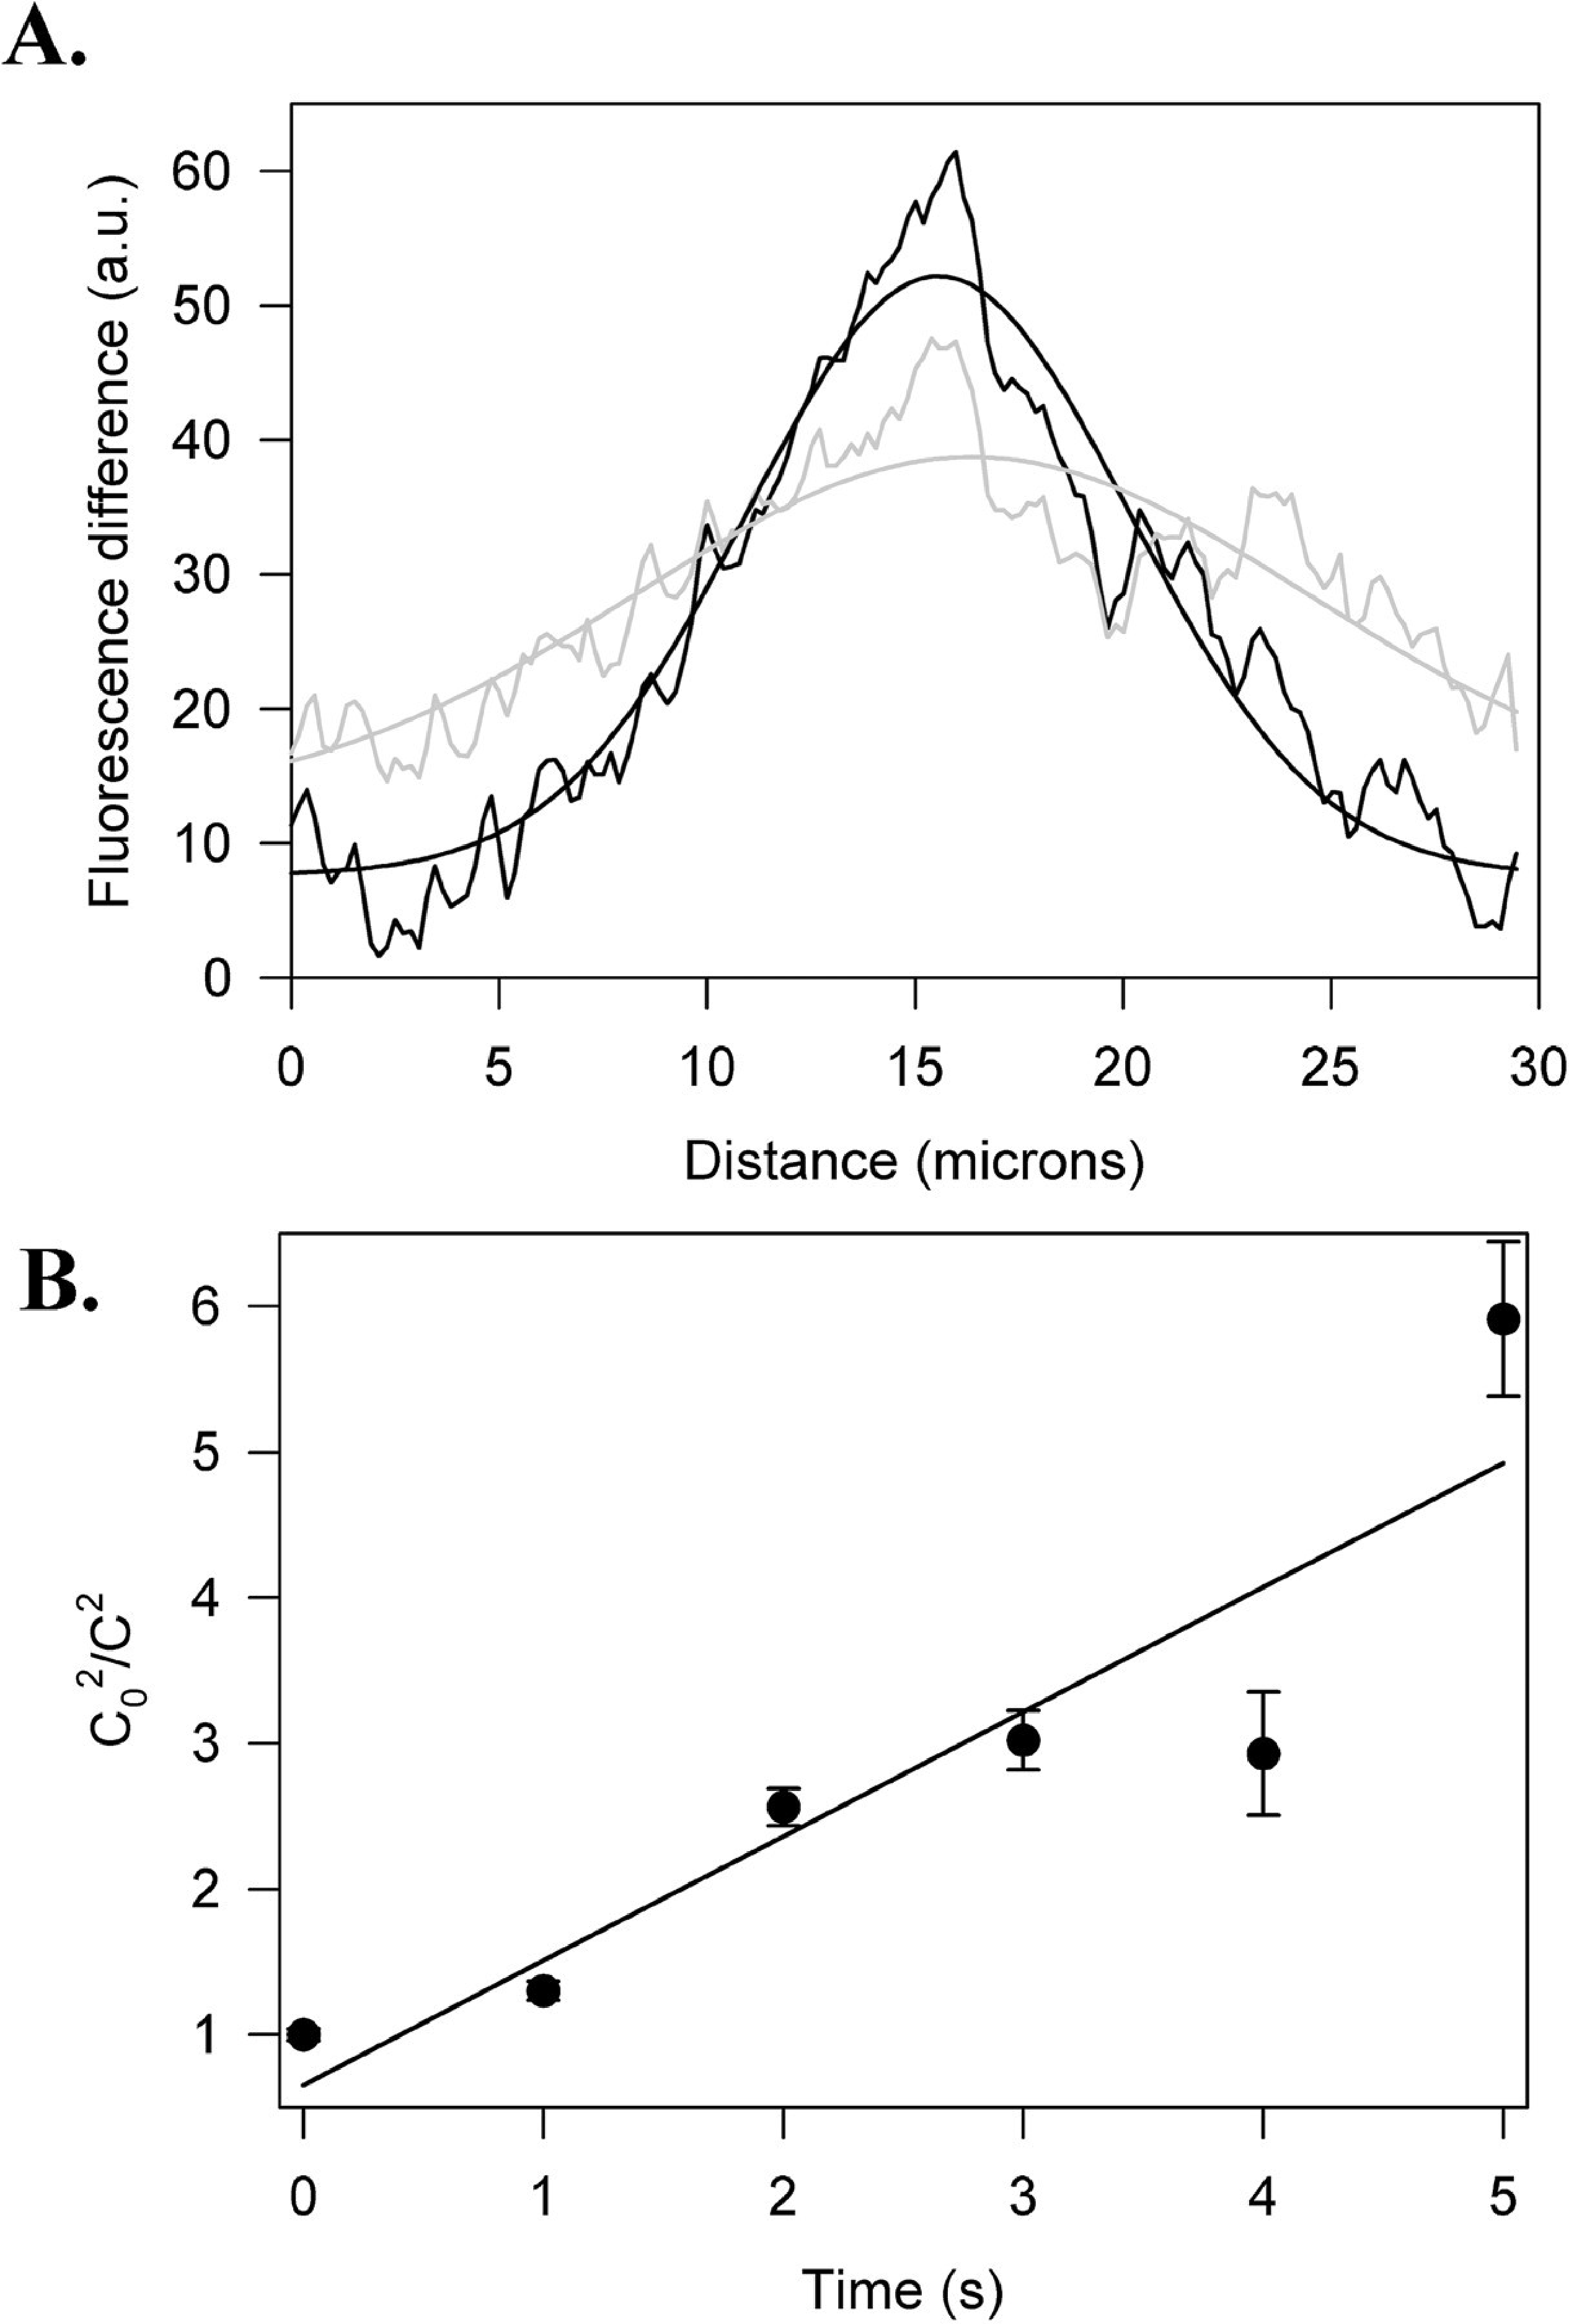
\includegraphics[trim = 10mm 300mm 00mm 30mm, clip, height=50mm]{F6_large.pdf}

Your goal is to write down an equation modeling the concentration of
protein over time. We'll split this problem up into two weeks. This
week: what PDE will you use to model the system? What are your initial
conditions? What are your boundary conditions? Will you be expanding
your solution in terms of $\sin$ or $\cos$ functions?

\section{Boas \S13.4 (waves on a string)} 
13.4.2, 13.4.12 (Due Wednesday)

\end{document}
